\documentclass[english]{article}
\usepackage[T1]{fontenc}
\usepackage[latin9]{inputenc}
\usepackage{geometry}
\geometry{verbose,lmargin=3cm,rmargin=3cm}
\usepackage{amsmath}
\usepackage{graphicx}
\usepackage{setspace}
\onehalfspacing
\usepackage{babel}
\usepackage{cite}
\usepackage{rotating}
\usepackage{tikz}
\usepackage{pdflscape}

\begin{document}

%\begin{quote}
%\begin{spacing}{0.5}
%\begin{center}
%{\footnotesize{}UNIVERSITY OF CALIFORNIA, DAVIS}\\
%{\footnotesize{} DEPARTMENT OF COMPUTER SCIENCE}
%\par\end{center}{\footnotesize \par}
%\end{spacing}
%\end{quote}

%\rule[0.5ex]{1\columnwidth}{1pt}

\title{\huge{Using AlphaGo Zero Techniques to Play Tic-Tac-Toe, Connect Four and Chess: Crop Dusting with an F-18}}
%\rule[0.5ex]{1\columnwidth}{1pt}
\author{
Adrian Chmielewski-Anders, Kenan Nalbant, Parsoa Khorsand Rahimzadeh, Sadegh Shamsabardeh \\
\{achmielewski, kanalbant, pkhorsand, mshamsabardeh\}@ucdavis.edu
}
\date{}

\maketitle


\begin{abstract}
There has been much success with using deep neural networks combined
with various forms of tree search in order to play perfect knowledge, zero-sum
games. Most notable are the techniques of AlphaGo. However,
these techniques still rely on datasets of professional games for training.
Most recently, it has been demonstrated that it is possible to play Go at
the highest level, with no prior game datasets.
This is achieved through consolidating the policy and value networks into a single
network, and omitting the use of rollouts. This single policy and value network
in conjunction with a modified Monte-Carlo Tree Search algorithm has proven to
yield exceptional results. We try to use this approach to play
other games, namely tic-tac-toe, Connect Four, and chess.

\end{abstract}
\section{Introduction}
The history of creating AI for game-playing dates far back. There have been many
efforts to create superhuman AI to play various board games. Most well-known
perhaps is that of IBM's Deep Blue. Previously, many of these methods relied on
quality of heuristic functions in order to evaluate board states.

Recently, due to the surge in development and progress of neural networks and
specifically deep neural networks has given rise to using neural networks in
conjunction with hand-crafted data--for example games of professional play--in
order to abstract out the handmade heuristic functions.
Training deep neural network with reinforcement learning have outperformed
human in computer games such as Atari and 3D virtual environments
\cite{eight, nine, ten}. There have been some efforts in the literature by
scholars to implement chess based on the reinforcement learning. In
\cite{one, two, three} the authors propose the reinforcement learning for 
self-play and the training is done based on temporal difference learning.
The authors have used handcrafted input features and these features
can be the source of performance limitation. \cite{one} and \cite{two} deploy pre-existing
computer programs as training opponents which limits the best achievable
performance. 

Additionally, there have been efforts which demonstrate that using deep neural
networks in conjunction with Q-learning can surpass humans at playing select
Atari video games \cite{DQN}. However, the game of Go remained unsolved in terms
of the ability of comptuers to play at professional human levels. This is due
to the very large board size ($19 \times 19$) which led many previous algorithms
to perform suboptimally. However, in recent years techniques involving using
neural networks for evaluating quality of board states and move possibilities
trained on games of professional play--the techniques behind AlphaGo--defeated the
European Go champion and later Lee Sedol--winner of 18 world titles--in a series
of 5 games in 2016 where AlphaGo won 4-1 \cite{AlphaGo, deepmind}.

The large state space of the chess together with the
aforementioned problems has led us to try using AlphaGo Zero techniques
to address these problems. This algorithm solves the problem
of large state space by exploring only those states that have more
probability of wining. To our best knowledge this is the first work
implementing AlphaGo Zero algorithm for the game of Chess.

We first attempt to play tic-tac-toe and Connect Four before moving on to chess.


%On the other hand, the reinforcement learning systems can learn on
%   their own based on their experiences and by taking random actions.
%   This characteristic makes them capable of surpassing human knowledge.
%   Reinforcement learning has recently drawn the attentions of researchers
%   and industries due to their promising capacities. These systems have
%   demonstrated better performance than human in some domains.
%   Training deep neural network with reinforcement learning have outperformed
%   human in computer games such as Atari and 3D virtual environments
\cite{eight, nine, ten}.
%   There have been some efforts in the literature by
%   scholars to implement chess based on the reinforcement learning. In
%   \cite{one, two, three} the authors propose the reinforcement learning for 
%   self-play and the training is done based on temporal difference learning.
%   The authors have used handcrafted input features and these features
%   can be the source of performance limitation. \cite{one} and \cite{two} deploy pre-existing
%   computer programs as training opponents which limits the best achievable
%   performance. The large state space of the chess together with the
%   above-mentioned problems makes our team to mimic the AlphaGo Zero
%   algorithm, developed by Google Deep Mind for the Game of Go, as reasonable
%   solution to address these problems. This algorithm solves the problem
%   of large state space by exploring only those states that have more
%   probability of wining. To our best knowledge this is the first work
%implementing AlphaGo Zero algorithm for the game of Chess. The following
%sections of this paper are organized as follow: \dots . 

\section{Methods}

The majority of the method is taken from \cite{AlphaGoZero} although key pieces
are modified so as to allow the method to work for other games such as chess.
These differences are noted throughout.

\subsection{Holistic Model}

The goal is to build a system which will output which action $a$ to make at a
give game state $s_t$. To do this, a variant of Monte-Carlo Tree Search (MCTS)
is used wherein the neural
network $f_{\theta}$ is used to guide the search. In the initial
game tree, the root node $s_0$ has no children. Such a node (while having
children since there exists legal actions from this state) is referred to as a
leaf node, distinct from a terminal node (one where there does not exist any
legal action resulting in a next state). To make a move, the MCTS starts with a
tree of just one node. Since it is a leaf node, it is expanded. Its children,
that is the next legal states, are added to the tree after feeding the states
through the neural network and obtaining $(p, v) = f_{\theta}(s)$ where $p$ is a
vector of move probabilities and $v$ is a scalar representing the value of the
state. In our modified version, both are scalars and we achieve a vector of $v$
values by feeding a combination of the current state and next states into the
network, resulting in more than one call to $f_{\theta}$. The values $p$ and $v$
are propagated through the tree, and the search is repeated. The MCTS operation
walks down the tree and makes decisions as to where to go based upon $p$ and $v$
as well as the visit count $N$. After many searches, the MCTS returns a
probability distribution $\pi$ based on the move count $N$. Based on $\pi$ a
move is selected as the move to make.

MCTS may therefore be viewed as a policy enhancement operator. The goal of the
method is to create data via games of self-play and to train the network based
on the true policy, the result of many MCTS searches, and the true value, the
winner of the game. Repeating this in the policy
iteration procedure is the strength of the AlphaGo Zero method. In
other words, the neural network parameters are updated to make the
probability $p$ and value $v$ be as close as possible to the search
probability $\pi$ and actual game winner $z$, respectively.

\subsection{Training}
Each iteration of the training is composed of playing $X$ games of self-play. Each game is composed of actions that are
performed based on probability $\pi$ from the starting state $s_{0}$
to the terminal state $s_{T}$. To take an action the MCTS search
Algorithm simulates moves many times and then perform the move
based on $\pi$. The simulation starts at current state $s_0$ and ends
at a leaf node $s_{L}$ by doing $L$ moves. At each time step $t<L$
of the simulation, an action is selected according to search tree
parameters and formula \ref{eq:1}. Emphasizing here that the actual
move of the game is not being played here and it is just a simulation
of the move. For each move that is made, the values $(s_t, \pi_t, z_t)$ are stored.
Where $s_t$ is the state at timestep $t$, $\pi_t$ is the output of the MCTS at
timestep $t$ and $z_t$ is 1 if the player at timestep $t$ wins or -1 if the
player loses.

At the end of each iteration, a sample of all $(s, \pi, z)$ values are sampled
uniformly and split into batches. From $s$ $(p, v) = f_{\theta}(s)$ are
obtained. For $E$ epochs, the network is trained on these batches. At fixed
number of iterations, a checkpoint occurs. Here, the previous best network,
$f_{\theta}^{\ast}$ is played against the current, recently trained network
$f_{\theta}$ over many games, if the current player wins more than 55\% of the
games, it is used in the next iteration, otherwise, the previous
$f_{\theta}^{\ast}$
is used. Many iterations are run until good performance is achieved. Figure
\ref{fig:figure_training} depicts a single iteration of training.


\begin{figure}[h]
\centering
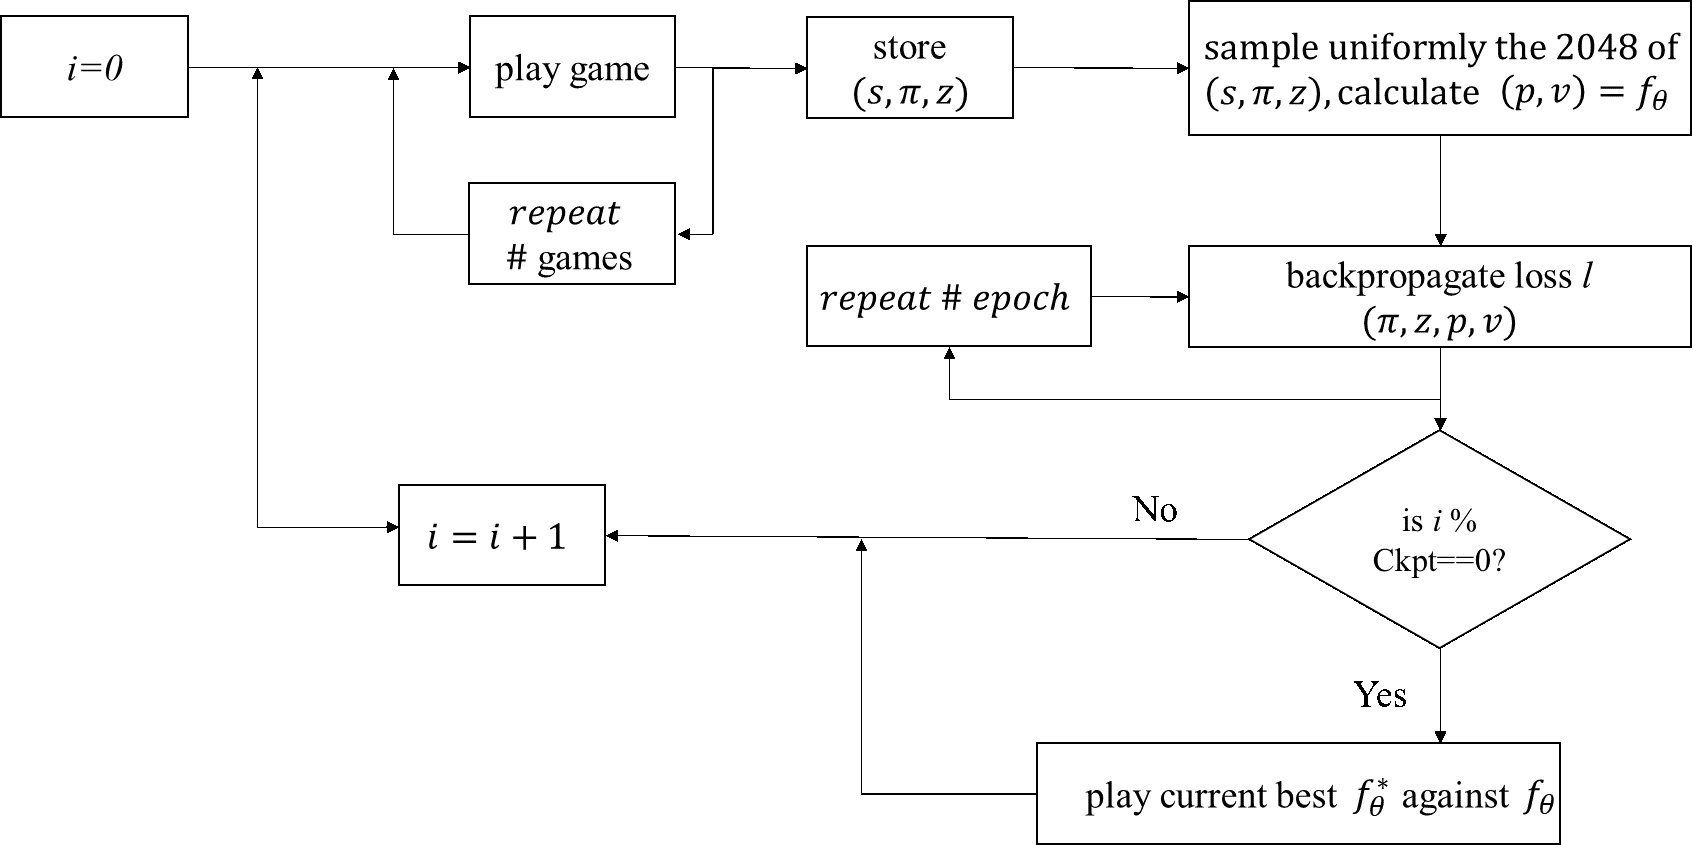
\includegraphics[scale=0.2]{./images/training}
\caption{What occurs during a single iteration of training. A series of games
    are played to generate data. The data is sampled uniformly, and the neural
    network is trained over many epochs on this data. At fixed poits, a
    checkpoint occurs and we evaluate the performance of the current player
    against the prevous best to determine which to use for future data
    generation.}
\label{fig:figure_training}
\end{figure}

\subsection{Self play}
During training, at each iteration many games of self-play are generated. For
each move in each game, the tree maintained by MCTS is shared among both
players, since they are the same. Moves are sampled from the probabilities $\pi$
returned by the MCTS search. That is $a_t \textasciitilde \pi$. After each iteration, the
network is trained based on the loss function
\begin{equation}
l=(z-v)^2 - \pi^T \log p
    \label{eq:3}
\end{equation}
Figure \ref{fig:figure_self_play} depicts what happens at one game of
self-play.
Note that we experimented with this loss function as $v$ is the average of $v$
for all forward operations.

\begin{figure}[h]
\centering
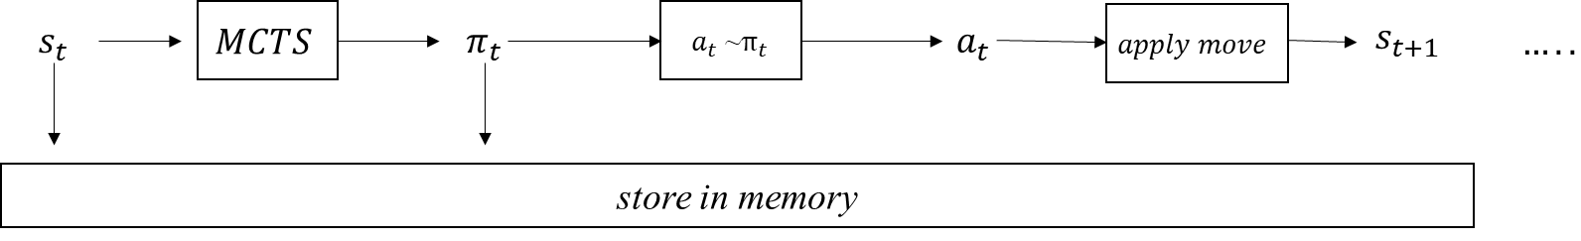
\includegraphics[width=0.7\textwidth]{./images/self_play}
\caption{How a move is made when training. A MCTS search is applied using the
    current network $f_{\theta}$ to expand a leaf node, if one is reached, edge
    values are modified, and $\pi_t$ is generated, an action is sampled from
    $\pi_t$ and applied. The process is repeated for all moves to generate data
    for a single game.}
\label{fig:figure_self_play}
\end{figure}

\subsection{Evaluator}
At fixed iteration intervals in the training process, we evaluate the current
neural network, with the previous best $f_{\theta}^{\ast}$. When the two play
against each other, they do not share the game tree maintained by MCTS.
Moreover, the moves $a_t$ are not sampled from $\pi$ but instead

\begin{equation}
    a_t=\underset{a}{\text{argmax}} (\pi_t)
\end{equation}

If the player using the current network wins more than 55\% of the games, it is
used for subsequent iterations. If not, the previous best is used.




\subsection{Search Algorithm of MCTS-Simulation}

In each position $s$ an MCTS search is executed during which the
tree is expanded. The following flow chart depicts the steps taken
by MCTS at each state $s$ of the game before making an actual action.

\begin{figure}[h]
\centering
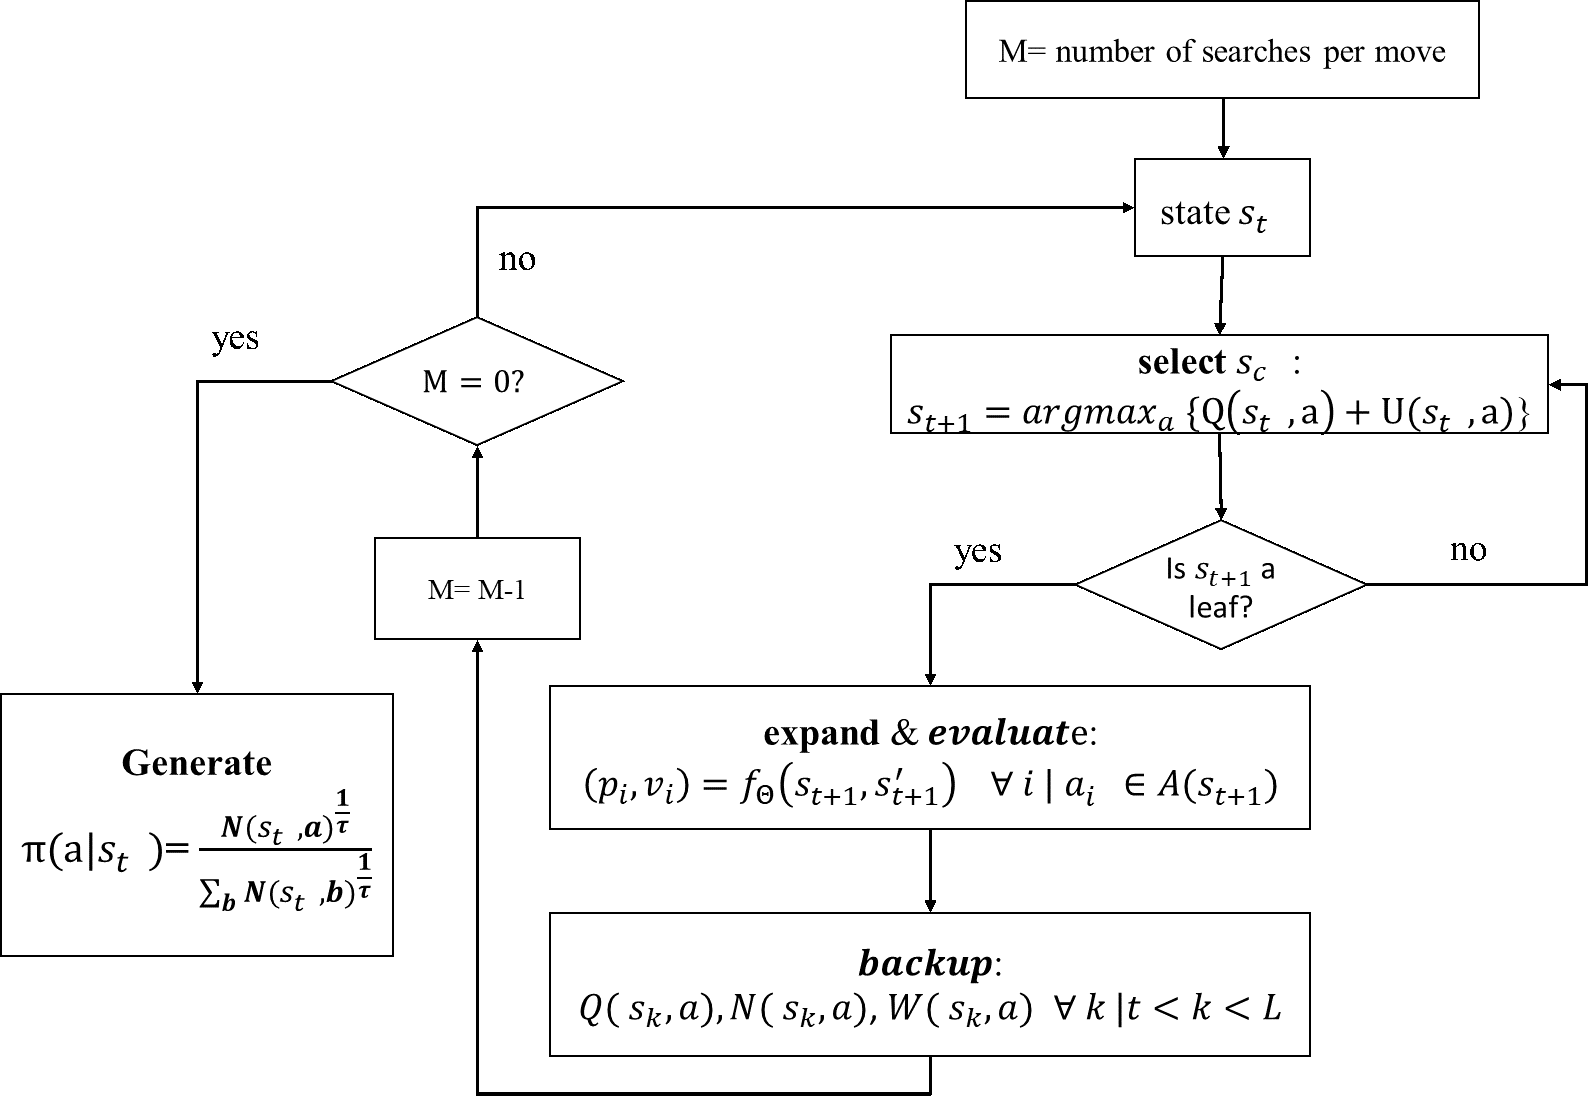
\includegraphics[width=0.7\textwidth]{./images/mcts}
\caption{Select: Each simulation traverses the tree by selecting the edge with
maximum action-value $Q$, plus an upper confidence bound $U$ that
depends on a stored prior probability $P$ and visit count $N$ for
that edge (which is incremented once traversed). Expand \& Evaluate:
The leaf node is expanded and the associated positions is evaluated
by the neural network $(P(s,\cdot),V(s))=f_{\theta}(s)$ ; the vector
of $P$ values are stored in the outgoing edges from $s$. Backup: Action-values
$Q$ are updated to track the mean of all evaluations $V$ in the
subtree below that action. play Once the search is complete, search
probabilities $\pi$ are returned, proportional to $N^{\frac{1}{\tau}}$,
where $N$ is the visit count of each move from the root state and
$\tau$ is a parameter controlling temperature.}
\label{fig:figure_mcts}
\end{figure}

MCTS begins with a root node $s_0$. In training, the game tree is shared across
both players so it is most likely expanded. That is, has children. If playing,
then it is an empty tree. MCTS walks down the tree and selects for each state at
time $s_t$ an action $a_t$ where
\begin{equation}
a_t=\underset{a}{\text{argmax}}(Q(s_{t},a)+U(s_{t},a))\label{eq:1}
\end{equation}
and
\begin{equation}
U(s,a)=c_{\text{puct}}P(s,a)\frac{\sqrt{\sum_{b}N(s,b)}}{1+N(s,a)},\label{eq:2}
\end{equation}


The selection procedure is based on the following parameters stored
at each edge $(s,a)$ of the tree. The visit count $N(s,a)$, the
total action-value $W(s,a)$, the mean action-value $Q(s,a)$, and
the prior probability of selecting that edge $P(s,a)$ . These values
are stored for all legal actions $a\in A(s)$ from $s$.  where $c_{\text{puct}}$
is a constant determining the level of exploration \cite{puct}.
Initially the visit counts are small numbers and the $U$ plays the
key role comparing to $Q$; the nodes with higher prior probability
are visited. However, this method asymptotically prefers actions with
high action-value. In other words, initially it explores more and
asymptotically it exploits more. 


Once the search reaches a
leaf node at time $L$ its children are added to the tree, with initial values

$$W(s_L, a_i) = 0, N(s_L, a_i) = 0, Q(s_L, a_i) = 0, P(s_L, a_i) = p_i$$

Then, all edges $t \leq L$ are updated with
$$N(s_t,a)=N(s_t,a)+1,W(s_t,a)=W(s_t,a)+v, Q(s_t,a)=\frac{W(s_t,a)}{N(s_t,a)}$$

Where $p$ and $v$ come from feeding the state through the network. Note here
that since we obtain a $v$ value for every call to the network, we replace $v$
with the average of all $v$ that we obtain.

If $s_L$ is a terminal node and cannot be expanded. All edges $t\leq L$ have
visit counts incremented and mean activation value adjusted
$Q(s_L,a)=\frac{W(s_L,a)}{N(s_L,a)}$. This procedure is done a fixed number of
times. Then $\pi$ is generated, where
$$\pi(a|s_0) = \frac{N(s_0,a)^{1/\tau}}{\sum_b N(s_0,b)^{1/\tau}}$$

Here $\tau$ is a temperature parameter. It is set to 1 for the first 30 moves of
the game, and then is set to be small, $\tau \rightarrow 0$. Again, this favors
exploration over exploitation earlier on in the game.


\subsection{Neural Network Architecture}
The network is similar to the one defined in the paper, although scaled down for
tic-tac-toe and Connect Four. It may be seen in four parts, one convolutional
block, followed by some number of residual blocks \cite{Residual} and the two outputs,
the policy and value heads.
For example, in tic-tac-toe, the following architecture was used:
The convolutional block is comprised of: 10 convolutional filters with dimension
$3 \times 3$ with stride 1, Batch Normalization, Relu. 
A residual block is comprised of: 10 convolutional filters with dimension
$3 \times 3$ with stride 1, Batch Normalization, Relu, 10 convolutional filters
with dimension $3 \times 3$ with stride 1, Batch Normalization, Output of Batch
Normalization is added to the input of the residual block.
The policy head consists of 2 convolutional filters of dimension $1 \times 1$
with stride 1, Batch Normalization, Relu, A fully connected layer to a single
output value, A nonlinearity (we experimented with sigmoid and softmax).

The value head consists of, 1 convolutional filter of dimension $1 \times 1$,
Batch Normalization, Relu, Fully connected layer of 16 output units, Relu,
Fully connected layer to a single output value, Tanh.

The input to all convolutional layers are padded so that the input height and
width match the output height and width.

\begin{figure}
	\centering
    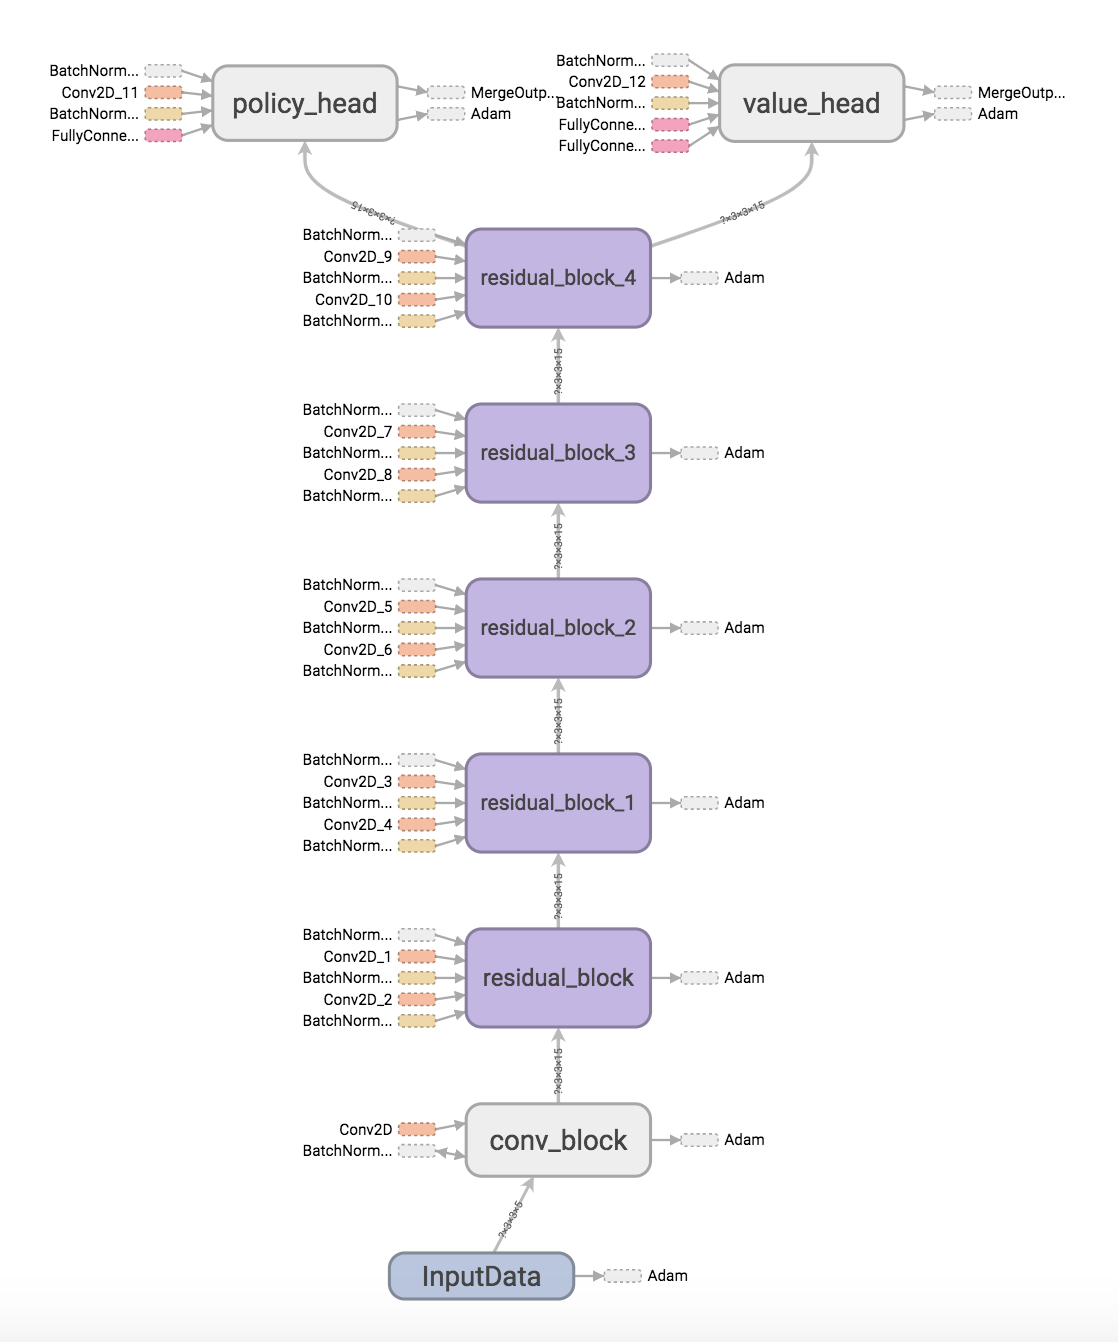
\includegraphics[scale=0.12]{network}
    \caption{Our network for tic-tac-toe with 5 residual blocks, in TensorFlow.}
\end{figure}


We cannot replicate the exact network that is used in \cite{AlphaGo} because
each output unit simply corresponds to placing a piece in that position. In
chess, we cannot accept this paradaigm for encoding a move and instead give to
the input a pair of states, which represent a a move from the current state to
the next state. The output of the network is two scalars $(p, v)$ which are
combined with other calls to the network for all possible moves to create $p$ a
vector, and $v$ a scalar which averages over all $v$.

Due to this change, the original loss function does not work since the original
loss function relies on $p$ being a probability distribution so the loss
function does not make as much sense. We instead also experimented with a more
simple MSE loss function, defined as follows
$$l=(z-v)^2+(p-\pi)^2$$
where all variables are scalars.

We also attempted to use the collection of $p$ values from the output of our
network, and feed this collection through a softmax, and the collection of $v$
values through an average function. Here we tried to approximate more closely
what is in the original paper, as we now have a true distribution over all
possible actions.
\section{Results}

We were not able to achieve great success with using the methods described above
in playing tic-tac-toe, Connect Four or chess. While it can be seen that over
time the ELO score for our player increases, it does not achieve super human
ability and can be beaten without too much effort. Although, it does not puerly
make poor moves. It, for example, consistently picks good initial positions for
tic-tac-toe and occasionally--depending on training parameters--for Connect
Four. Across all games, it seems able to make good attack moves, although does
not seem able to play defensively very well. For example, in Connect Four, a
common scenario is having three in a row for both players. Our player will often
give up a win by not blocking the opponents winning row or column. 

While not as interpretable as some standard supervised machine learning
problems, we can see that our model does reduce error over time, as seen in
figure \ref{fig:lossMSE}. Moreover, in figure \ref{fig:lossMSE} we can see that the original
error function for our model is extremely noisy and our model does not learn
from it.

\begin{figure}
\centering
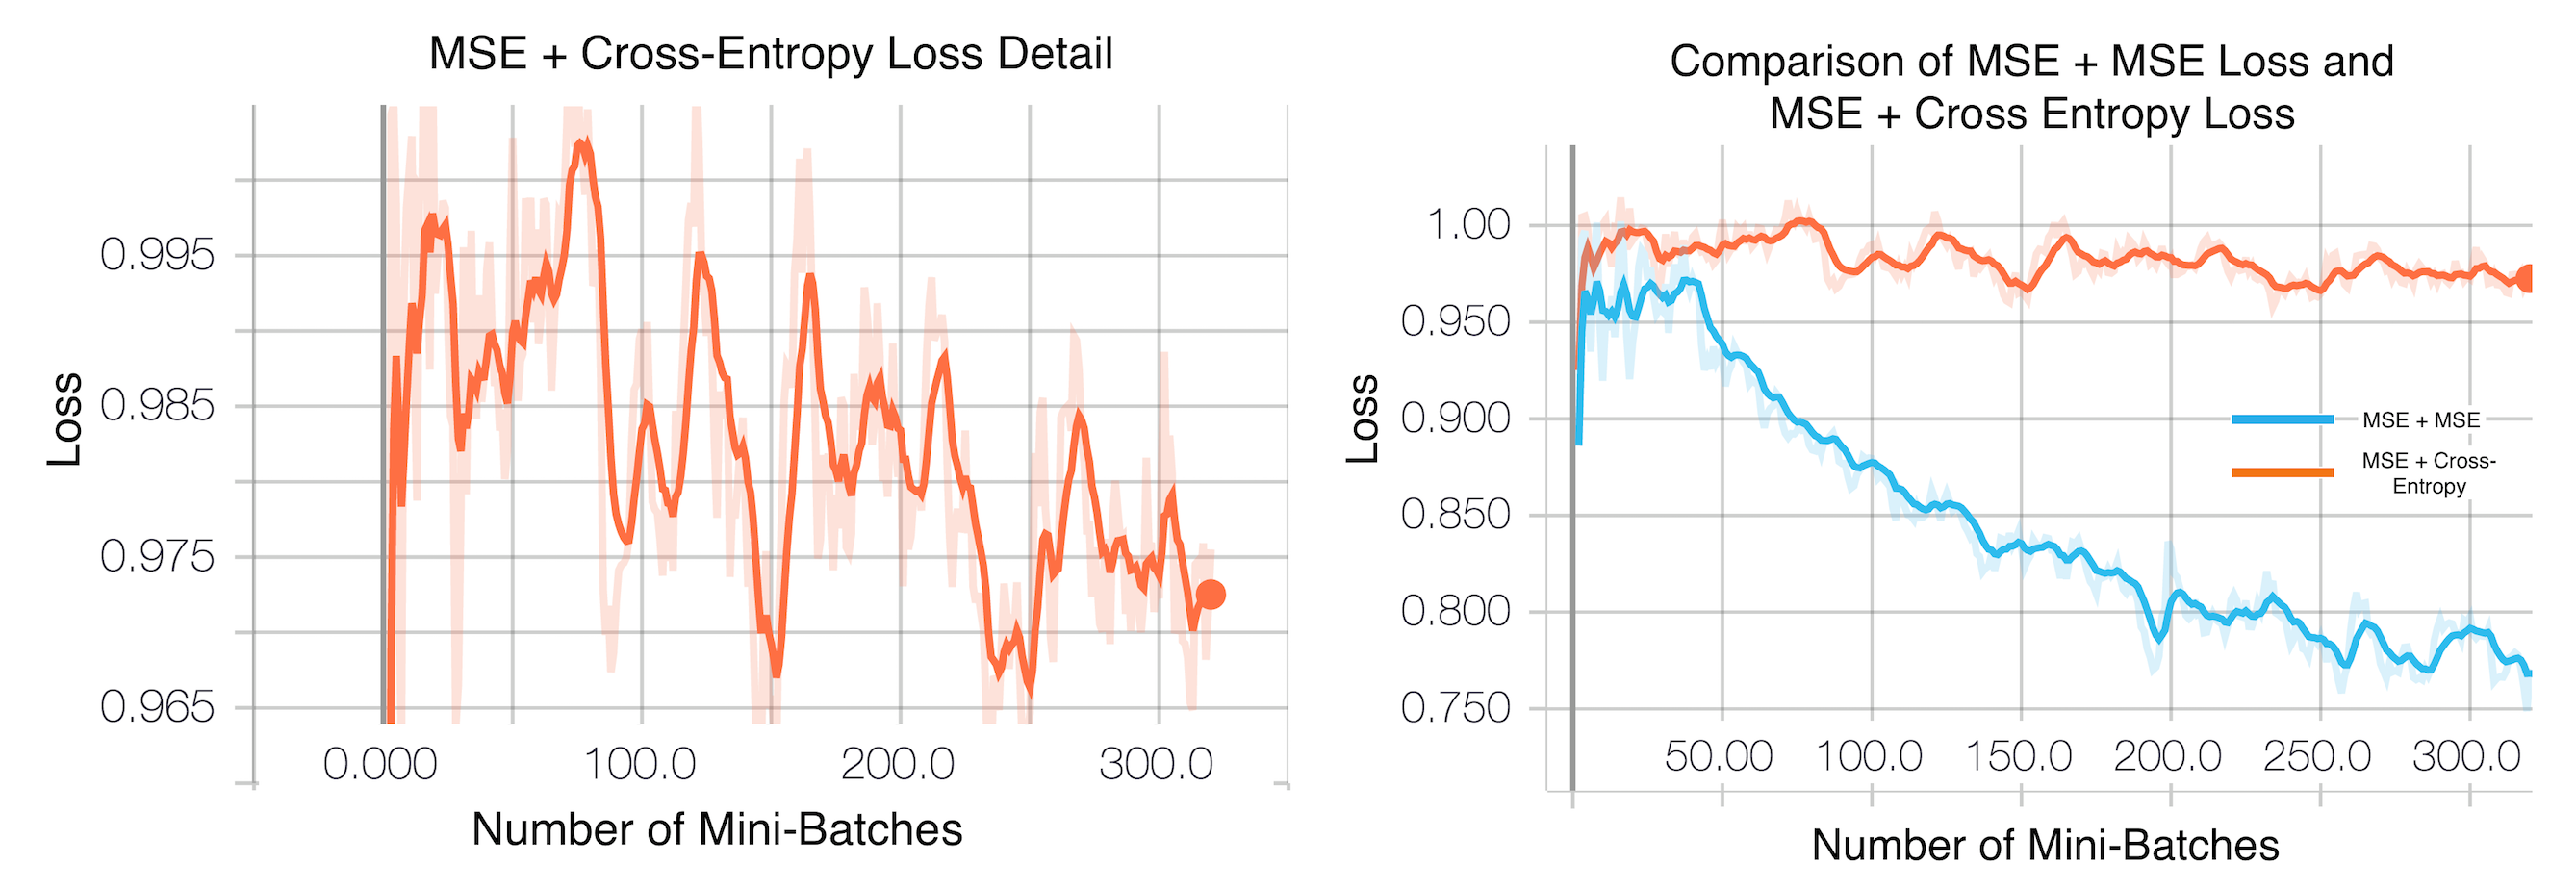
\includegraphics[width=\textwidth]{plots}
    \label{fig:lossMSE}
    \caption{\textbf{Right}: The modified MSE loss function compared with the original MSE and
    Cross-Entropy. Due to our modifications, the original loss function did not
    capture quality of moves. \textbf{Left}: The original loss function with our modifications is very noisy.}
\end{figure}


\subsection{Performance}

Performance of the trained models was evaluated using the Elo\cite{Elo} rating
system, the same measure used by the AlphaGo Zero paper. The details and
inner-workings of the Elo algorithm are beyond the scope of this paper. We
trained the model for each game for a number of iterations and ranked each
iteration through a series of games with the previous iterations and a random
player. The random player simply picks moves at random and was incorporated to
provide a baseline for the Elo rating of the first iteration. Ranking of an
iteration is adjusted once all the games have finished and once an iteration is
rated, it rating will be frozen for the rest of the evaluation. Based on the
system used by the FIDE \cite{Elo} to rank players with no prior history, each player (including the random player) will start with the Elo score of 750. 

The graphs below depict the improvement in the model's playing performance over time. As expected, the Elo rating of the model increases (although not strictly) with training time.

\begin{figure}[h]
\centering
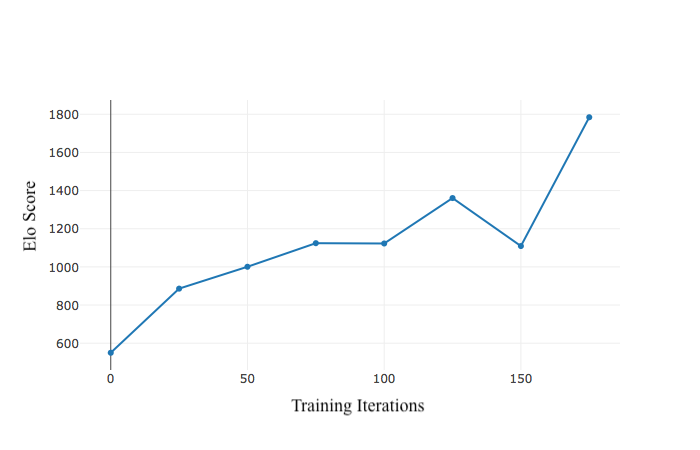
\includegraphics[width=0.7\textwidth]{./images/ttt}
\caption{The performance of the model trained for the tic-tac-toe game over time}
\label{fig:figure_ttt}
\end{figure}

\section{Discussion}
We experienced a myriad of difficulties in reproducing the success of the paper
in other games.
Initially, we tried to model the paper as close as possible and used the
original loss function \ref{eq:3}. This did not work given the changes we made
to the network output. Additionally it can be seen that this loss function is
very noisy given our modifications.
We also suspect that even though we use scaled down versions of the networks,
that they are still quite large, and we did not have access to enough
computational power in order to train our models over a large enough set of
games. Moreover, we experienced problems with parameter tuning as there are well
in excess of 15 different hyperparameters and we expect that to get a model
which works very well that we would need to spend more resources on tuning these
parameters to the games in question. We also suspect that our modifications to
the output of the network in order to allow for playing chess resulted in
considering all possible moves for a given state independently of one another
and this perhaps resulted in our model making poor moves.

Future work might entail exploration of how these techniques fare with other
games apart from just Go. Work like this is imoprtant because it advances the
field generally and helps in udnerstanding what more advanced algorithms are
capable of.

\clearpage
\bibliography{references}
\bibliographystyle{IEEEtran}

\section{Author contributions}
Adrian Chmielewski-Anders: Game infrastructure, game and network cohesion, report writing.\\
Kenan Nalbant: Network design, network infrastructure, game infrastructure, data generation.\\
Parsoa Khorsand Rahimzadeh: MCTS implementation, Elo rating and evaluation, code debugging, data generation, report writing.\\
Sadegh Shamsabardeh: Majority of paper writing, move playing infrastructure
\end{document}
